\documentclass{article}

\usepackage[margin=0.5in]{geometry}
\usepackage{multicol}
\usepackage{graphicx}
\usepackage{tkz-euclide}
\usepackage{amsmath}
\usepackage{amsthm}

\theoremstyle{definition}
\newtheorem*{solution}{Solution}
\title{Problem-Solving Set B}
\author{}
\date{}

\begin{document}
\maketitle
\begin{multicols*}{2}
    \begin{enumerate}
        \item A bar graph shows the number of hamburgers sold by a fast food chain each season.
            However, the bar indicating the number sold during the winter is covered by a smudge.
            If exactly $25\%$ of the chain's hamburgers are sold in the fall, how many million hamburgers are sold in the winter?
            \begin{center}
                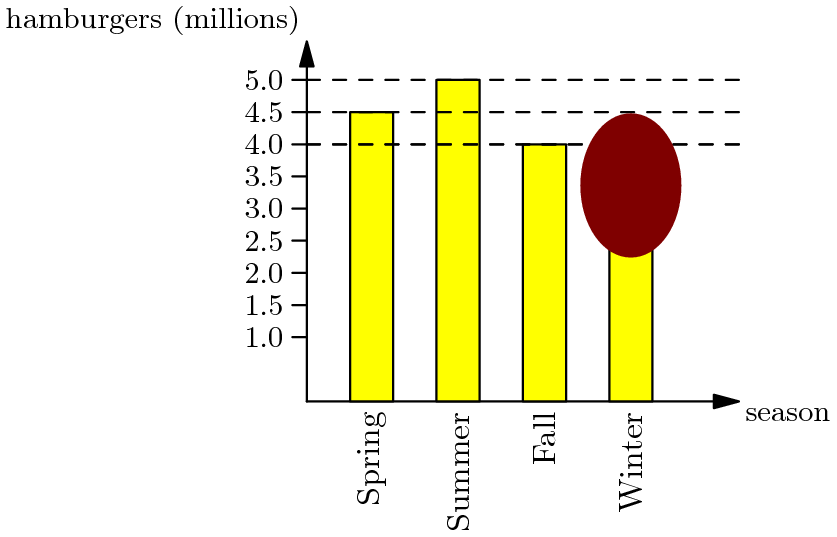
\includegraphics[scale=0.2]{5-2_bar_graph.png}
            \end{center}
            \begin{solution}
                What we want to find is the number of hamburgers sold in the winter.
                Since we don't know what it is, let's call it $x$.
				From the graph, we know that $4.5$ million hamburgers were sold in the spring, $5$ million in the summer, and $4$ million in the fall.
                We know that the number of hamburgers sold in the fall is exactly $\frac{1}{4}$ of the total number of hamburgers sold, so we can say that:
                \begin{align*}
                    4 \times \text{Fall} &= \text{Spring} + \text{Winter} + \text{Fall} + \text{Summer} \\
                    4 \times 4 &= 4.5 + 4 + x + 5 \\
                    16 &= x + 13.5 \\
                    2.5 &= x
                \end{align*}
            \end{solution}
        \item Suppose only one of the eight lettered identical squares is included with the four squares in the T-shaped figure outlined.
            How many of the resulting figures can be folded into a topless cubical box?
            \begin{center}
                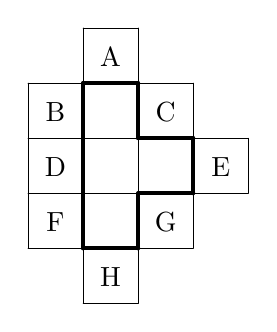
\begin{tikzpicture}[scale=0.7]
                    \foreach \xcoord\ycoord\name in {0/1/A1, 0/4/A2, 1/0/B1, 1/5/B2, 2/0/C1, 2/5/C2, 3/1/D1, 3/4/D2, 4/2/E1, 4/3/E2, 0/2/F1, 0/3/F2}
                    {
                        \tkzDefPoint(\xcoord,\ycoord){\name}
                    }
                        
                    \tkzDrawSegments(A1,A2 B1,B2 C1,C2 D1,D2 E1,E2)
                    \tkzDrawSegments(B2,C2 A2,D2 F2,E2 F1,E1 A1,D1 B1,C1)

                    \foreach \x\y\d\z\name in {B1/B2/A2/D2/I1, C1/C2/A2/D2/I2, C1/C2/F2/E2/I3, D1/D2/F2/E2/I4, D1/D2/F1/E1/I5, C1/C2/F1/E1/I6, C1/C2/A1/D1/I7, B1/B2/A1/D1/I8, B1/B2/F2/E2/J2, B1/B2/F1/E1/J1}
                    {
                        \tkzInterLL(\x,\y)(\d,\z)
                        \tkzGetPoint{\name}
                    }
                    \tkzDrawSegments[line width = 0.5mm](I1,I2 I2,I3 I3,I4 I4,I5 I5,I6 I6,I7 I7,I8 I8,I1)
                    \foreach \x\y\name in {B2/C2/A, A2/I1/B, I2/D2/C, F2/J2/D, I4/E2/E, F1/J1/F, I6/I5/G, I8/I7/H}
                    {
                        \tkzLabelSegment[below, yshift=-3.5](\x,\y){\name}
                    }
                \end{tikzpicture}
            \end{center}
            \begin{solution}
                Fold the four squares into four sides of a cube.
                Then, there are six unconnected edges.
                For each open edge, we can add a square/side, so the answer is $6$.
            \end{solution}
        \item If $A$ and $B$ are nonzero digits, how many digits does the sum of these three numbers have?
			\[
				\begin{array}{ccccc}
					  & 9 & 8 & 7 & 6 \\
					  &   & A & 3 & 2 \\
					+ &   &   & B & 1 \\
					\hline
				\end{array}
			\]
            \begin{solution}
                The minimum possible value of this sum is when $A = B = 1$, which is $9876 + 132 + 11 = 10019$.
                The largest possible value of the sum is when $A = B = 9$, making the sum $9876 + 932 + 91 = 10899$.
                Since all the possible sums re between $10019$ and $10899$, they must have $5$ digits.
            \end{solution}
        \item $ABCD$ is a rectangle, $D$ is the center of the circle, and $B$ is on the circle.
            If $AD = 4$ and $CD = 3$, then the area of the shaded region is between which two integers?
            \begin{center}
                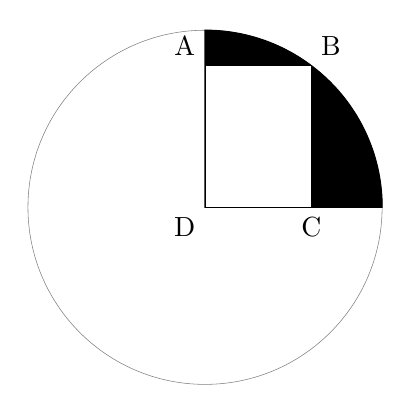
\begin{tikzpicture}[scale=0.45]
                    \tkzDefPoint(0,0){D}
                    \tkzDefPoint(0,4){A}
                    \tkzDefPoint(3,4){B}
                    \tkzDefPoint(3,0){C}
                    \tkzDefPoint(0,5){E}
                    \tkzDefPoint(5,0){F}

                    \tkzDrawCircle(D,B)
                    \tkzDrawSector[fill=black](D,F)(E)

                    \tkzDrawPolygon[fill=white](D,A,B,C)
                    \tkzLabelPoint[above left](A){A}
                    \tkzLabelPoint[above right](B){B}
                    \tkzLabelPoint(C){C}
                    \tkzLabelPoint[below left](D){D}
                \end{tikzpicture}
            \end{center}
            \begin{solution}
                The area of the shaded region is equal to the area of the quarter circle minus the area of the rectangle.
                The area of the rectangle is $4 \cdot 3 = 12$, so we just need the quarter circle.
                Applying the Pythagorean Theorem to $\triangle ADC$, we have $(AC)^2 = 4^2 + 3^2 \rightarrow AC = 5$.
                Since $ABCD$ is a rectangle, $BD = AC = 5$.
                Clearly $BD$ is a radius of the circle, so the area of the whole circle is $\pi 5^2 = 25\pi$ and the area of the quarter circle is $\frac {25\pi}{4}$, which is between $7$ and $8$.
            \end{solution}
        \item A palindrome is a whole number that reads the same forwards and backwards.
            If one neglects the colon, certain times displayed on a digital watch are palindromes.
            Three examples are $1\colon 01$, $4\colon 44$, and $12\colon 21$.
            How many times during a $12$-hour period will be palindromes?
            \begin{solution}
                From $1$ to $9$, the times will be of the form $a\colon ba$.
                There are $9$ choices for $a$ and $6$ choices for $b$, so there are $9 \cdot 6 = 54$ times in this period.
                From $10$ to $12$, the minutes are already determined, so there are only $3$ times in this case.
                In total, there are $57$ palindromic times.
            \end{solution}
    \end{enumerate}
\end{multicols*}
\end{document}
